
\documentclass[a4paper,11pt]{article}
\usepackage[a4paper, margin=8em]{geometry}

% usa i pacchetti per la scrittura in italiano
\usepackage[french,italian]{babel}
\usepackage[T1]{fontenc}
\usepackage[utf8]{inputenc}
\frenchspacing 

% usa i pacchetti per la formattazione matematica
\usepackage{amsmath, amssymb, amsthm, amsfonts}

% usa altri pacchetti
\usepackage{gensymb}
\usepackage{hyperref}
\usepackage{standalone}

\usepackage{colortbl}

\usepackage{xstring}
\usepackage{karnaugh-map}

% imposta il titolo
\title{Electronics for Embedded Systems notes}
\author{Luca Seggiani}
\date{2026}

% spaziatura liste
\usepackage{enumitem}
\setlist[itemize]{noitemsep, topsep=4pt, partopsep=0pt, parsep=2pt, leftmargin=*}
\setlist[enumerate]{noitemsep, topsep=4pt, partopsep=0pt, parsep=2pt, leftmargin=*}

% imposta lo stile
% usa helvetica
\usepackage[scaled]{helvet}
% usa palatino
\usepackage{palatino}
% usa un font monospazio guardabile
\usepackage{lmodern}

\renewcommand{\rmdefault}{ppl}
\renewcommand{\sfdefault}{phv}
\renewcommand{\ttdefault}{lmtt}

% circuiti
\usepackage{circuitikz}
\usetikzlibrary{babel}

% testo cerchiato
\newcommand*\circled[1]{\tikz[baseline=(char.base)]{
            \node[shape=circle,draw,inner sep=2pt] (char) {#1};}}

% disponi il titolo
\makeatletter
\renewcommand{\maketitle} {
	\begin{center} 
		\begin{minipage}[t]{.8\textwidth}
			\textsf{\huge\bfseries \@title} 
		\end{minipage}%
		\begin{minipage}[t]{.2\textwidth}
			\raggedleft \vspace{-1.65em}
			\textsf{\small \@author} \vfill
			\textsf{\small \@date}
		\end{minipage}
		\par
	\end{center}

	\thispagestyle{empty}
	\pagestyle{fancy}
}
\makeatother

% disponi teoremi
\usepackage{tcolorbox}
\newtcolorbox[auto counter, number within=section]{theorem}[2][]{%
	colback=blue!10, 
	colframe=blue!40!black, 
	sharp corners=northwest,
	fonttitle=\sffamily\bfseries, 
	title=Theorem~\thetcbcounter: #2, 
	#1
}

% disponi definizioni
\newtcolorbox[auto counter, number within=section]{definition}[2][]{%
	colback=red!10,
	colframe=red!40!black,
	sharp corners=northwest,
	fonttitle=\sffamily\bfseries,
	title=Definition~\thetcbcounter: #2,
	#1
}

% disponi codice
\usepackage{listings}
\usepackage[table]{xcolor}

\definecolor{codegreen}{rgb}{0,0.6,0}
\definecolor{codegray}{rgb}{0.5,0.5,0.5}
\definecolor{codepurple}{rgb}{0.58,0,0.82}
\definecolor{backcolour}{rgb}{0.95,0.95,0.92}

\lstdefinestyle{codestyle}{
		backgroundcolor=\color{black!5}, 
		commentstyle=\color{codegreen},
		keywordstyle=\bfseries\color{magenta},
		numberstyle=\sffamily\tiny\color{black!60},
		stringstyle=\color{green!50!black},
		basicstyle=\ttfamily\footnotesize,
		breakatwhitespace=false,         
		breaklines=true,                 
		captionpos=b,                    
		keepspaces=true,                 
		numbers=left,                    
		numbersep=5pt,                  
		showspaces=false,                
		showstringspaces=false,
		showtabs=false,                  
		tabsize=2
}

\lstdefinestyle{shellstyle}{
		backgroundcolor=\color{black!5}, 
		basicstyle=\ttfamily\footnotesize\color{black}, 
		commentstyle=\color{black}, 
		keywordstyle=\color{black},
		numberstyle=\color{black!5},
		stringstyle=\color{black}, 
		showspaces=false,
		showstringspaces=false, 
		showtabs=false, 
		tabsize=2, 
		numbers=none, 
		breaklines=true
}

\lstdefinelanguage{x86}{ 
  keywords={AAA, AAD, AAM, AAS, ADC, ADCB, ADCW, ADCL, ADD, ADDB, ADDW, ADDL, AND, ANDB, ANDW, ANDL,
        ARPL, BOUND, BSF, BSFL, BSFW, BSR, BSRL, BSRW, BSWAP, BT, BTC, BTCB, BTCW, BTCL, BTR, 
        BTRB, BTRW, BTRL, BTS, BTSB, BTSW, BTSL, CALL, CBW, CDQ, CLC, CLD, CLI, CLTS, CMC, CMP,
        CMPB, CMPW, CMPL, CMPS, CMPSB, CMPSD, CMPSW, CMPXCHG, CMPXCHGB, CMPXCHGW, CMPXCHGL,
        CMPXCHG8B, CPUID, CWDE, DAA, DAS, DEC, DECB, DECW, DECL, DIV, DIVB, DIVW, DIVL, ENTER,
        HLT, IDIV, IDIVB, IDIVW, IDIVL, IMUL, IMULB, IMULW, IMULL, IN, INB, INW, INL, INC, INCB,
        INCW, INCL, INS, INSB, INSD, INSW, INT, INT3, INTO, INVD, INVLPG, IRET, IRETD, JA, JAE,
        JB, JBE, JC, JCXZ, JE, JECXZ, JG, JGE, JL, JLE, JMP, JNA, JNAE, JNB, JNBE, JNC, JNE, JNG,
        JNGE, JNL, JNLE, JNO, JNP, JNS, JNZ, JO, JP, JPE, JPO, JS, JZ, LAHF, LAR, LCALL, LDS,
        LEA, LEAVE, LES, LFS, LGDT, LGS, LIDT, LMSW, LOCK, LODSB, LODSD, LODSW, LOOP, LOOPE,
        LOOPNE, LSL, LSS, LTR, MOV, MOVB, MOVW, MOVL, MOVSB, MOVSD, MOVSW, MOVSX, MOVSXB,
        MOVSXW, MOVSXL, MOVZX, MOVZXB, MOVZXW, MOVZXL, MUL, MULB, MULW, MULL, NEG, NEGB, NEGW,
        NEGL, NOP, NOT, NOTB, NOTW, NOTL, OR, ORB, ORW, ORL, OUT, OUTB, OUTW, OUTL, OUTSB, OUTSD,
        OUTSW, POP, POPL, POPW, POPB, POPA, POPAD, POPF, POPFD, PUSH, PUSHL, PUSHW, PUSHB, PUSHA, 
        RCLL, RCR, RCRB, RCRW, RCRL, RDMSR, RDPMC, RDTSC, REP, REPE, REPNE, RET, ROL, ROLB, ROLW,
        ROLL, ROR, RORB, RORW, RORL, SAHF, SAL, SALB, SALW, SALL, SAR, SARB, SARW, SARL, SBB,
        SBBB, SBBW, SBBL, SCASB, SCASD, SCASW, SETA, SETAE, SETB, SETBE, SETC, SETE, SETG, SETGE,
        SETL, SETLE, SETNA, SETNAE, SETNB, SETNBE, SETNC, SETNE, SETNG, SETNGE, SETNL, SETNLE,
        SETNO, SETNP, SETNS, SETNZ, SETO, SETP, SETPE, SETPO, SETS, SETZ, SGDT, SHL, SHLB, SHLW,
        SHLL, SHLD, SHR, SHRB, SHRW, SHRL, SHRD, SIDT, SLDT, SMSW, STC, STD, STI, STOSB, STOSD,
        STOSW, STR, SUB, SUBB, SUBW, SUBL, TEST, TESTB, TESTW, TESTL, VERR, VERW, WAIT, WBINVD,
        XADD, XADDB, XADDW, XADDL, XCHG, XCHGB, XCHGW, XCHGL, XLAT, XLATB, XOR, XORB, XORW, XORL},
  keywordstyle=\color{blue}\bfseries,
  ndkeywordstyle=\color{darkgray}\bfseries,
  identifierstyle=\color{black},
  sensitive=false,
  comment=[l]{\#},
  morecomment=[s]{/*}{*/},
  commentstyle=\color{purple}\ttfamily,
  stringstyle=\color{red}\ttfamily,
  morestring=[b]',
  morestring=[b]"
}

\lstdefinelanguage{riscv}{
  keywords={
    LUI, AUIPC,
    JAL, JALR,
    BEQ, BNE, BLT, BGE, BLTU, BGEU,
    LB, LH, LW, LBU, LHU, LD,
    SB, SH, SW, SD,
    ADDI, SLTI, SLTIU, XORI, ORI, ANDI,
    SLLI, SRLI, SRAI,
    ADD, SUB, SLL, SLT, SLTU, XOR, SRL, SRA, OR, AND,
    ADDIW, SLLIW, SRLIW, SRAIW,
    ADDW, SUBW, SLLW, SRLW, SRAW,
    MUL, MULH, MULHSU, MULHU, DIV, DIVU, REM, REMU,
    MULW, DIVW, DIVUW, REMW, REMUW,
    LR.W, SC.W, AMOSWAP.W, AMOADD.W, AMOXOR.W,
    AMOAND.W, AMOOR.W, AMOMIN.W, AMOMAX.W,
    AMOMINU.W, AMOMAXU.W,
    LR.D, SC.D, AMOSWAP.D, AMOADD.D, AMOXOR.D,
    AMOAND.D, AMOOR.D, AMOMIN.D, AMOMAX.D,
    AMOMINU.D, AMOMAXU.D,
    FLW, FSW,
    FMADD.S, FMSUB.S, FNMSUB.S, FNMADD.S,
    FADD.S, FSUB.S, FMUL.S, FDIV.S, FSQRT.S,
    FSGNJ.S, FSGNJN.S, FSGNJX.S,
    FMIN.S, FMAX.S,
    FCVT.W.S, FCVT.WU.S, FCVT.S.W, FCVT.S.WU,
    FMV.X.W, FMV.W.X,
    FEQ.S, FLT.S, FLE.S,
    FLD, FSD,
    FMADD.D, FMSUB.D, FNMSUB.D, FNMADD.D,
    FADD.D, FSUB.D, FMUL.D, FDIV.D, FSQRT.D,
    FSGNJ.D, FSGNJN.D, FSGNJX.D,
    FMIN.D, FMAX.D,
    FCVT.W.D, FCVT.WU.D, FCVT.D.W, FCVT.D.WU,
    FCVT.S.D, FCVT.D.S,
    FMV.X.D, FMV.D.X,
    FEQ.D, FLT.D, FLE.D,
    CSRRW, CSRRS, CSRRC,
    CSRRWI, CSRRSI, CSRRCI,
    FENCE.I,
    FENCE,
    ECALL, EBREAK,
    MRET, SRET, URET,
    WFI,
    SFENCE.VMA,
    NOP, LI, LA, MV,
    NOT, NEG, NEGW,
    SEQZ, SNEZ, SLTZ, SGTZ,
    BEQZ, BNEZ, BLEZ, BGEZ, BLTZ, BGTZ,
    BGT, BLE, BGTU, BLEU,
    J, JR, RET,
    CALL, TAIL,
    RDINSTRET, RDCYCLE, RDTIME,
    CSRR, CSRW, CSRS, CSRC,
    CSRWI, CSRSI, CSRCI
  },
  keywordstyle=\color{blue}\bfseries,
  ndkeywordstyle=\color{darkgray}\bfseries,
  identifierstyle=\color{black},
  sensitive=false,
  comment=[l]{\#},
  morecomment=[s]{/*}{*/},
  commentstyle=\color{purple}\ttfamily,
  stringstyle=\color{red}\ttfamily,
  morestring=[b]',
  morestring=[b]"
}

\lstdefinelanguage{arm}{
  keywords={
    ADC, ADD, AND, BIC, CMN, CMP, EOR, MOV, MVN,
    RSB, RSC, SBC, SUB, TST, TEQ,
    MLA, MLS, MUL, SMLAL, SMULL, UMLAL, UMULL,
    QADD, QSUB, QDADD, QDSUB,
    QADD16, QADD8, QASX, QSAX,
    QSUB16, QSUB8, QSAX, QSUBADDX,
    ASR, LSL, LSR, ROR, RRX,
    B, BL, BX, BLX,
    BXJ,
    BEQ, BNE, BCS, BHS, BCC, BLO,
    BMI, BPL, BVS, BVC,
    BHI, BLS, BGE, BLT, BGT, BLE,
    BAL,
    LDR, LDRB, LDRH, LDRSB, LDRSH,
    LDRD, LDM, LDMIA, LDMIB, LDMDA, LDMDB,
    LDRT, LDRBT, LDRHT, LDRSBT, LDRSHT,
    STR, STRB, STRH, STRD,
    STM, STMIA, STMIB, STMDA, STMDB,
    STRT, STRBT, STRHT,
    PUSH, POP,
    SWP, SWPB,
    REV, REV16, REVSH,
    BFC, BFI, BFXIL, SBFX, UBFX,
    CLZ,
    LDREX, LDREXB, LDREXH, LDREXD,
    STREX, STREXB, STREXH, STREXD,
    DMB, DSB, ISB,
    MCR, MCRR, MRC, MRRC,
    MRS, MSR,
    CPS, SETEND, SVC, BKPT,
    CLREX, WFE, WFI, SEV,
    YIELD, NOP,
    VLDR, VSTR,
    VMOV, VABS, VNEG,
    VADD, VSUB, VMUL, VDIV,
    VMLA, VMLS, VNMLA, VNMLS, VNMUL,
    VMAX, VMIN,
    VSQRT,
    VCMP, VCMPE,
    VCVT,
    VCLZ, VCLS,
    VAND, VORR, VEOR, VBIC, VMVN,
    VLD1, VLD2, VLD3, VLD4,
    VST1, VST2, VST3, VST4,
    ADR, ADCS, ADDS, SUBS, MOVS, ANDS, ORRS, EORS
  },
  keywordstyle=\color{blue}\bfseries,
  ndkeywordstyle=\color{darkgray}\bfseries,
  identifierstyle=\color{black},
  sensitive=false,
  comment=[l]{@},
  morecomment=[l]{;},
  morecomment=[s]{/*}{*/},
  commentstyle=\color{purple}\ttfamily,
  stringstyle=\color{red}\ttfamily,
  morestring=[b]',
  morestring=[b]"
}

\lstset{style=codestyle, language=C}

% disponi sezioni
\usepackage{titlesec}

\titleformat{\section}
	{\sffamily\Large\bfseries} 
	{\thesection}{1em}{} 
\titleformat{\subsection}
	{\sffamily\large\bfseries}   
	{\thesubsection}{1em}{} 
\titleformat{\subsubsection}
	{\sffamily\normalsize\bfseries} 
	{\thesubsubsection}{1em}{}

% tikz
\usepackage{tikz}

% float
\usepackage{float}

% grafici
\usepackage{pgfplots}
\pgfplotsset{width=10cm,compat=1.9}

% disponi alberi
\usepackage{forest}

\forestset{
	rectstyle/.style={
		for tree={rectangle,draw,font=\large\sffamily}
	},
	roundstyle/.style={
		for tree={circle,draw,font=\large}
	}
}

% disponi algoritmi
\usepackage{algorithm}
\usepackage{algorithmic}
\makeatletter
\renewcommand{\ALG@name}{Algorithm}
\makeatother

% disponi numeri di pagina
\usepackage{fancyhdr}
\fancyhf{} 
\fancyfoot[L]{\sffamily{\thepage}}

\makeatletter
\fancyhead[L]{\raisebox{1ex}[0pt][0pt]{\sffamily{\@title \ \@date}}} 
\fancyhead[R]{\raisebox{1ex}[0pt][0pt]{\sffamily{\@author}}}
\makeatother

\begin{document}
% sezione (data)
\section{Lesson 25-09-26}

% stili pagina
\thispagestyle{empty}
\pagestyle{fancy}

% testo

In the last lesson we introduced the resistive load inverter.
We said that the main problem of such a design is the asymmetric response, and static power consumption (as in the output off state we have a closed path from power source to ground, draining power on a resistor).
Today we try to solve those problems.

\textbf{\textsf{CMOS inverter}}: a better inverter can be designed by using \textbf{Complementary} \textit{MOS} (\textbf{CMOS}) designs.

\begin{center}
	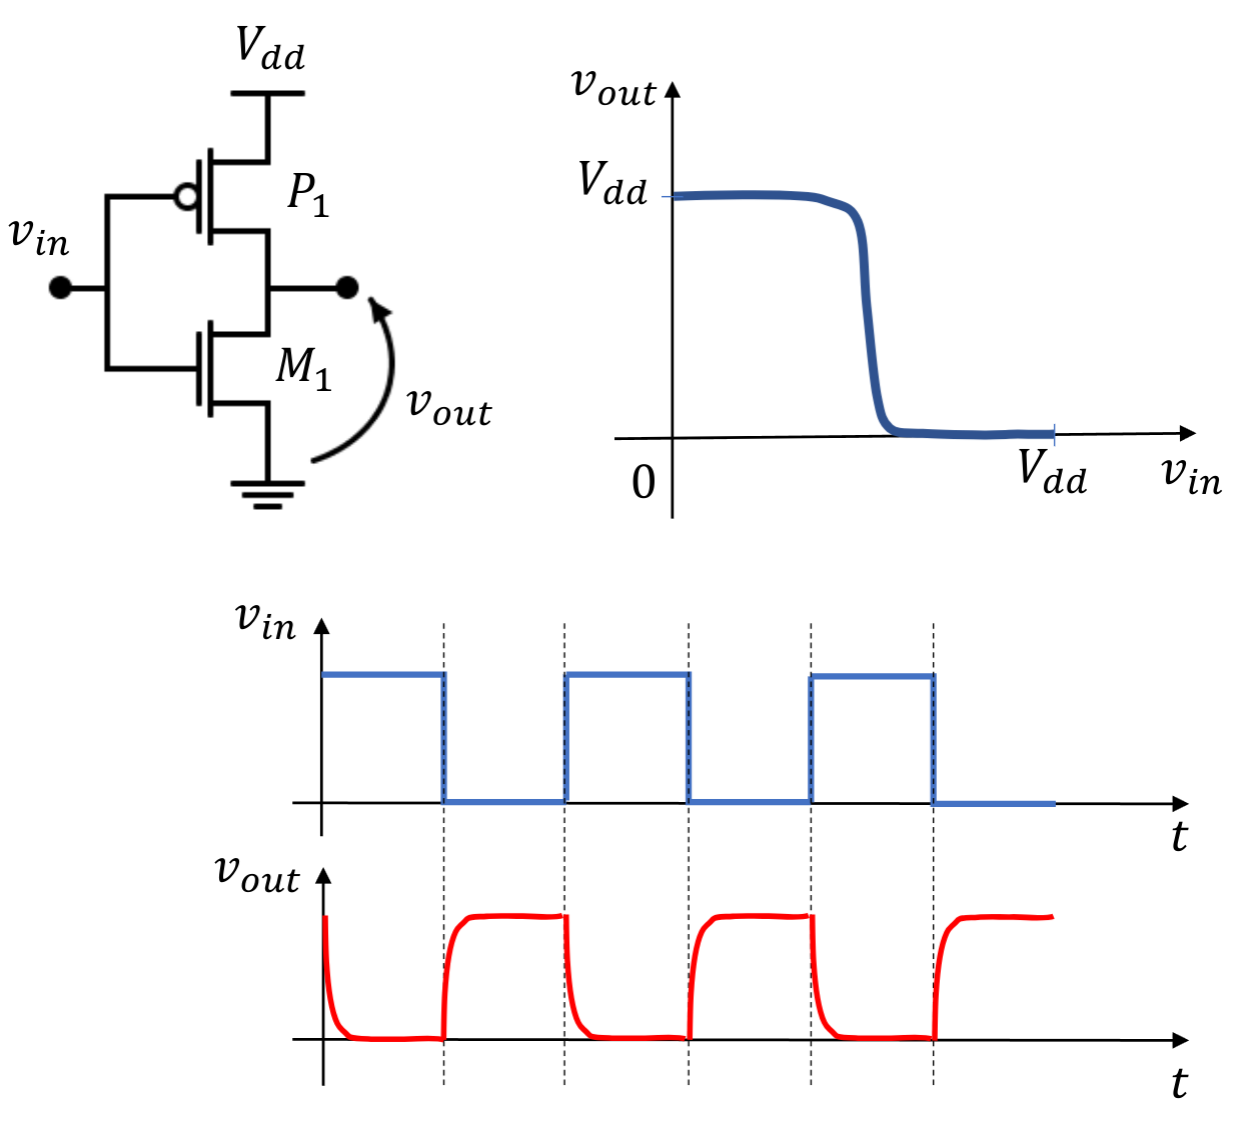
\includegraphics[scale=0.3]{../figures/cmos_inv.png}
\end{center}

We see that in such a design:
\begin{itemize}
	\item The response is \textbf{symmetric} (or mostly symmetric, we can act on the gate sizes to account for mobility effects);
	\item There is no \textbf{static} power consumption (in the ideal case, some leakage does happen);
	\item \textbf{Dynamic} power is present and measurable based on equivalent capacitance of the wire and the MOS transistors:
$$
P \approx C_{e1} f V^2
$$
\end{itemize}

This design is very common in digital circuits nowadays, as it performs much better than the resistive load inverter. 

\textbf{\textsf{CMOS logic}}: other logic functions are needed to implement a logic family.
For CMOS technolog, we can use combinations of transistors in series or in parallel to implement any kind of logic.

In particular:
\begin{itemize}
\item In the pull-down branch:
\begin{itemize}
\item Series NMOS implements a NAND
\item Parallel NMOS implements a NOR
\end{itemize}
\item In the pull-up branch:
\begin{itemize}
\item Series PMOS implements a NOR
\item Parallel PMOS implements a NAND
\end{itemize}
\end{itemize}

We show a figure of the synthesis of a NAND and NOR circuit in CMOS technology:
\begin{center}
	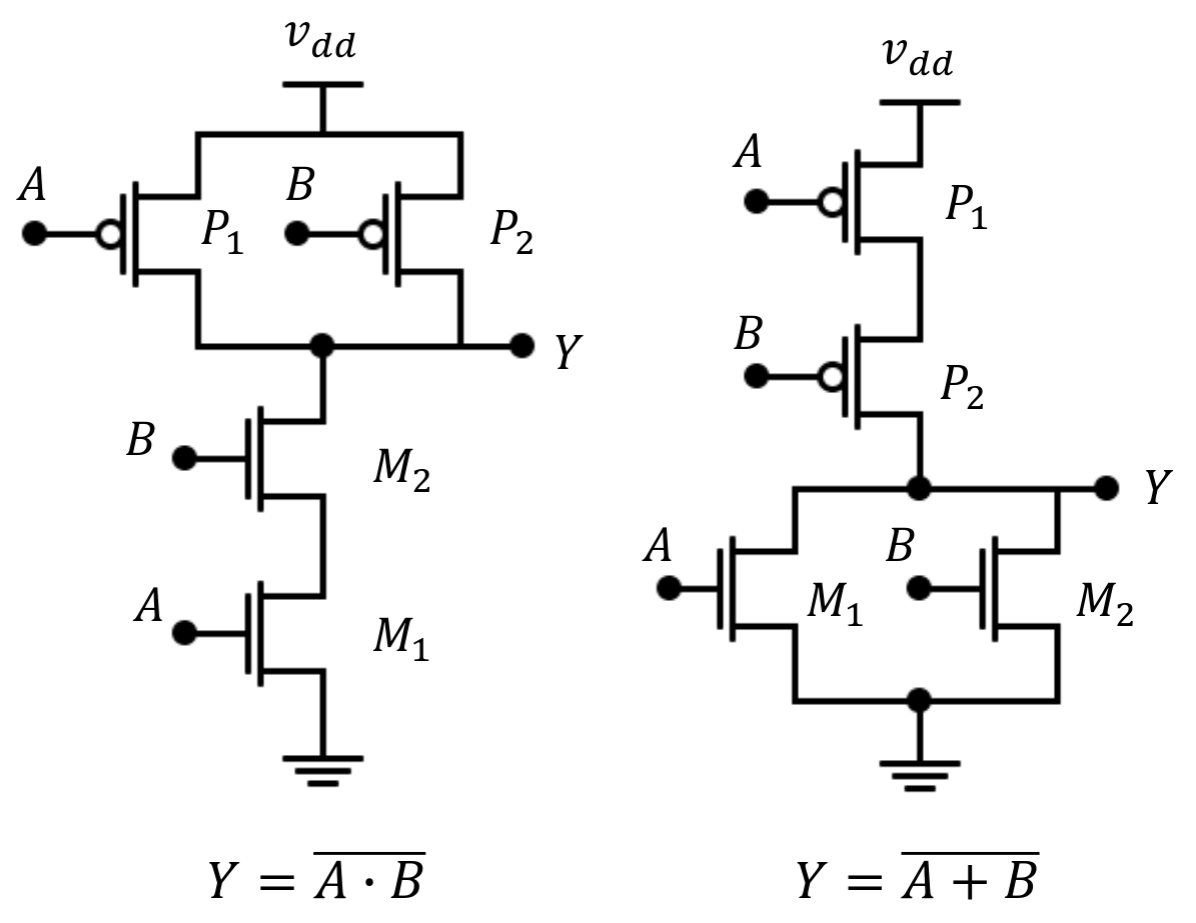
\includegraphics[scale=0.22]{../figures/cmos_nand_nor.png}
\end{center}

\textbf{\textsf{Logic gate parameters}}: we can define input and output parameters for logic gates, regarding both \textit{current} and \textit{voltage}.

With regards to \textbf{current}, we can model a CMOS inverter converting the MOS transistors to voltage controlled switches (ideal) with series resistances modeling leakage.
This way we see we can define the parameters:
\begin{itemize}
	\item $V_{OH}$, which is the lowest output voltage to get a logic high output;
	\item $V_{OL}$, which is the highest output voltage to get a logic low output;
	\item $I_{OH}$, which is the maximum output current such that the output voltage at logic high is greater than $V_{OH}$;
	\item $I_{OL}$, which is the maximum output current such that the output voltage at logic low is less than $V_{OL}$.
\end{itemize}

\begin{center}
	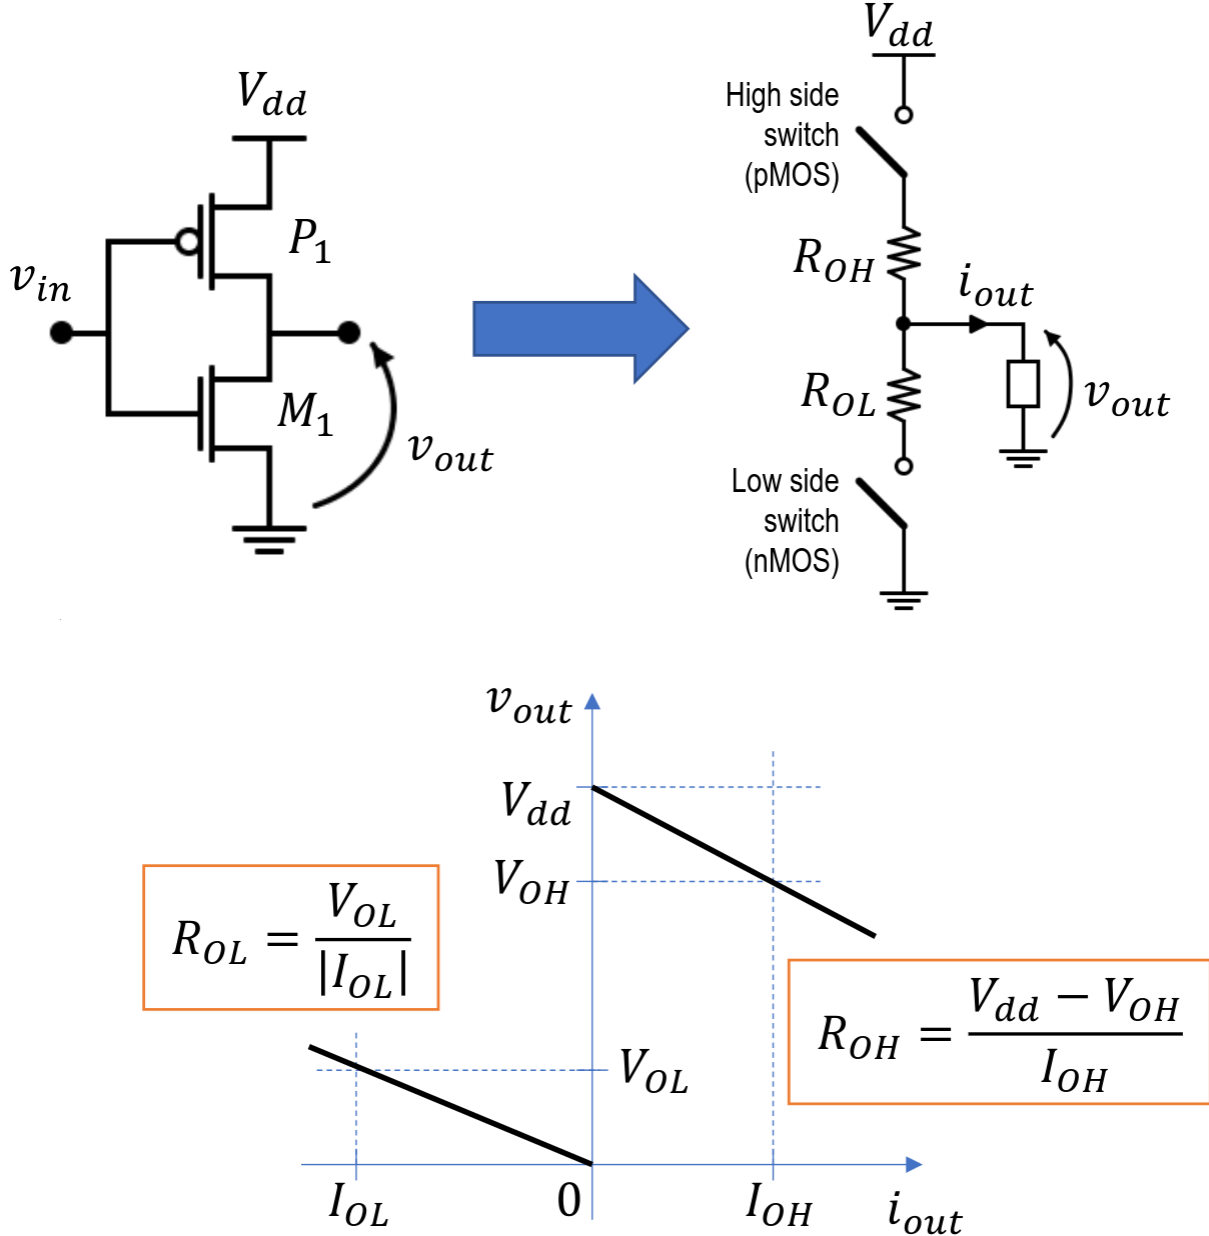
\includegraphics[scale=0.22]{../figures/current_io.png}
\end{center}

From these parameters (given by constructors) we can compute the value of the modeling resistances:
$$
R_{OL} = \frac{V_{OL}}{|I_{OL}|}
,\quad
R_{OH} = \frac{V_{dd} - V_{OH}}{I_{OH}}
$$

\par\smallskip

Now, with regards to input and output \textbf{voltages} in stacked gate setups, we can consider the following:

\begin{center}
	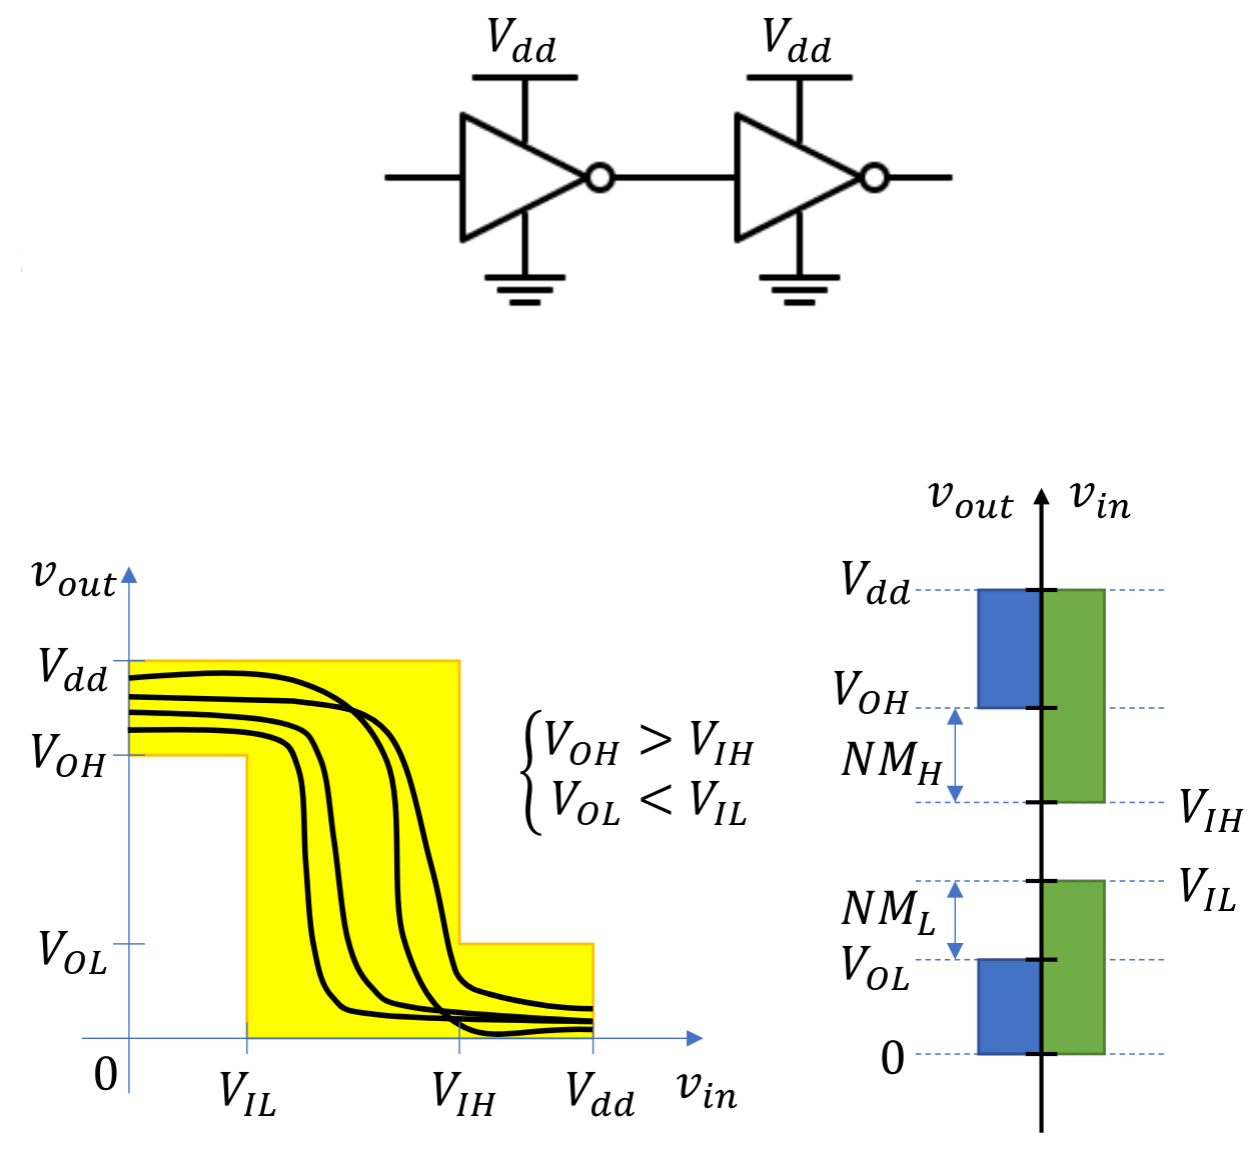
\includegraphics[scale=0.22]{../figures/voltage_io.png}
\end{center}

Here we have a pair of connected inverters.
We are interested on whether ouput voltages of the first inverter will be correctly interpreted at the input of the second inverter, so we define the following parameters:
\begin{itemize}
	\item $V_{IH}$, which is the lowest input voltage recognized as logic high;
	\item $V_{IL}$, which is the highest input voltage recognized as logic low;
\end{itemize}

From this we can derive stability \textit{conditions} for the whole logic family:
$$
V_{OH} > V_{IH}, \quad V_{OL} < V_{IL}
$$
where we define the following margins:
$$
V_{OH} - V_{IH} = NM_H \quad \text{(noise margin high)}
$$
$$
V_{IL} - V_{OL} = NM_L \quad \text{(noise margin low)}
$$

\textbf{\textsf{Tri-state}} outputs are needed to avoid logic gates shorting when connected to the same outputs.

In these designs we have an additional Enable input, which can be \textit{active high} or \textit{active low}:
\begin{itemize}
	\item When Enable is active, the output is driven normally;
	\item When Enable is NOT active, both the pull-up (high side) and pull-down (low side) transistors are switched OFF, and the output line is left floating.
		At this point the voltage level (and consequently the logic level) is set by some other circuit, or remains undetermined.
\end{itemize}

Below, we show the symbol of a tri-state inverter and a possible CMOS implementation.

\begin{center}
	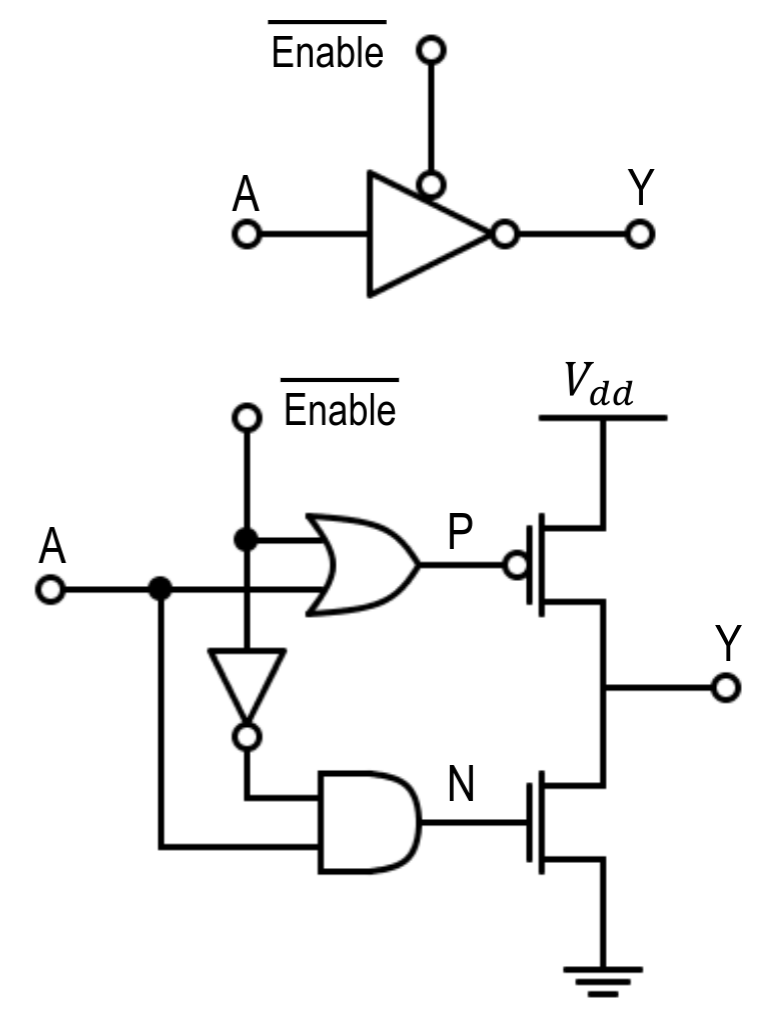
\includegraphics[scale=0.22]{../figures/tristate_inv.png}
\end{center}

As we said, tri-state outputs are useful when multiple logic gates drive the same line, for instance in a shared bus.
All drivers must be in high impedance except one: it is vital to guarantee the above condition to avoid short circuits.

\textbf{\textsf{Open collector}} is another technology which allows to drive the same data line, even without knowing the voltage supply value.

In this setup, there is no pull-up transistor at the output: we can only set the output to logic 0.
To set a logic 1, we switch off all pull-down transistors, and use an external pull-up resistor.

\begin{center}
	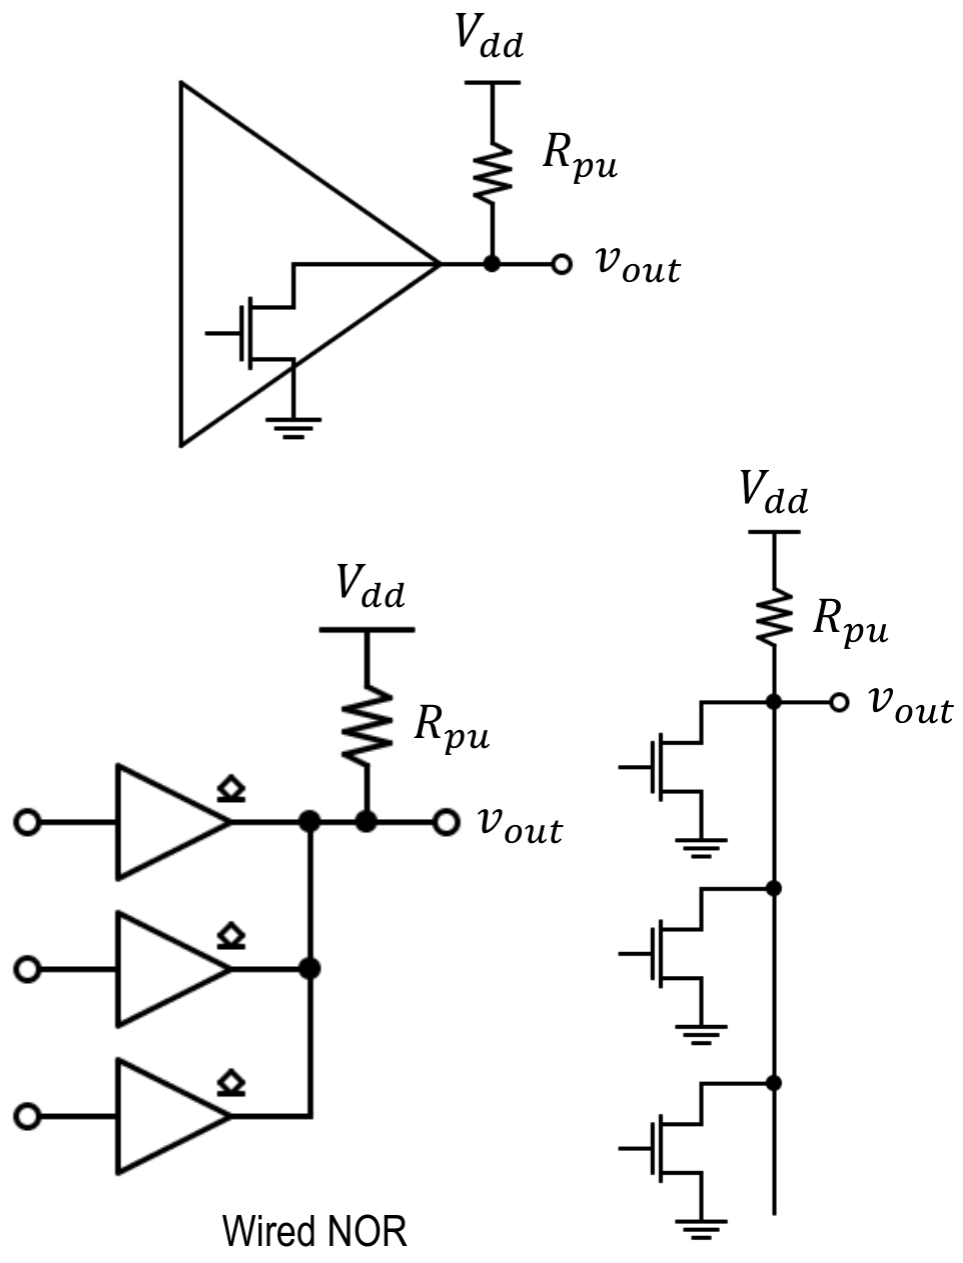
\includegraphics[scale=0.22]{../figures/open_collector.png}
\end{center}

This is useful to drive the same line with multiple logic gates:
\begin{itemize}
	\item No possible short circuit: when all logic gates set a logic 1 the output is at logic 1;
	\item When at least one logic gate sets a logic 0, the output goes at logic 0. This makes open collector a NOR logic function.
\end{itemize}

This is slighly easier to implement than the earlier tri-state solution, as we don't have to deal with high impedance or short circuit issues.

Of course, we can imagine an \textit{open drain} setup which works the same, only leaving the pull-down transistor outside of the design and pulling \textit{up} thorugh an external resistor.

\subsection{Combinatorial circuits}

\textbf{Combinatorial circuits} are the simplest we can see with digital logic circuits.
In a combinatorial logic circuit, the logic output depends on the current value of the inputs only (no state).

A combinatorial circuit can be described through a \textbf{truth table}, which is a list all possible input combinations, and corresponding output values.

Many ways exist to synthesize a combinatorial circuit:
\begin{itemize}
	\item The main idea is generally to generate the circuit as a \textbf{SoP} (\textit{Sum of Products}), minimizing the number of products, and minimizing the number of literals in each product (which corresponds to minimizing components).
	\item A possible tool is given by \textit{Karnaugh maps};
	\item Another possibility is the \textit{Quine-McCluskey algorithm} for more inputs;
	\item Often, we just stick to logic synthesis \textit{software tools}, which implement these ore other advanced algorithms.
\end{itemize}

\textbf{\textsf{Multiplexers}} are circuits which allow to select an input and output just one of them, between different inputs.
A one bit multiplexer with 2 inputs has this boolean law:
$$
y = a \cdot s + b \cdot \overline{s}
$$
where $a$ and $b$ are the inputs, and $s$ is the selection signal.

For multiplexers on multiple bits, we repeat the same structure multiple times;
For multiplexers with more than two inputs, we need more than one selection signal (usually built hierarchically with $\log{\text{number of inputs}}$ smaller multiplexers).
Multiplexers with more than two inputs on multiple bits are built as a combination of the above two cases.

\textbf{\textsf{Decoders}} decode the binary representation of a number, on $n$ bits, to the same number in one-hot representation, on $2^n$ bits.

\textbf{\textsf{Encoders}} do the reverse job of converting a one-hot representation on $2^n$ bits in a single $n$ bit encoded value.

More complex components like \textit{priority encoders}, ... can be built.

\textbf{\textsf{Digital adders / subtractors}} are built in combinatorial logic too.

We start from \textit{half adders}: these operate on 1-bit operands, generating a carrying output bit.
For \textit{multibit} adders we combine multiple half adders.

Different area and performance can be achieved based on carry computation.
For instance, we remember:
\begin{itemize}
\item Ripple Carry
\item Carry Look Ahead
\item Carry Select
\end{itemize}

\textit{Subtractors} are just implemented using an adder (using 2-complement notation).

\subsection{Sequential circuits}

\textbf{Sequential circuits} need a \textit{memory element} to exist somewhere in a circuit.
The most popoular memory element is given by a pair of active elements in a loop.
\begin{itemize}
	\item A pair of inverters in a loop provides a memory element, that is an element that is \textit{bistable}: either of the inverters can start out with an high outputs, and the state is converted. The problem of this design is that we can't control it:
	\item A pair of NANDS in a loop can be used in the same fashion. The input bits that are left out can be used as SET and RESET parameters for the bistable circuit. We call this a \textbf{SR latch}.
\end{itemize}

\begin{center}
	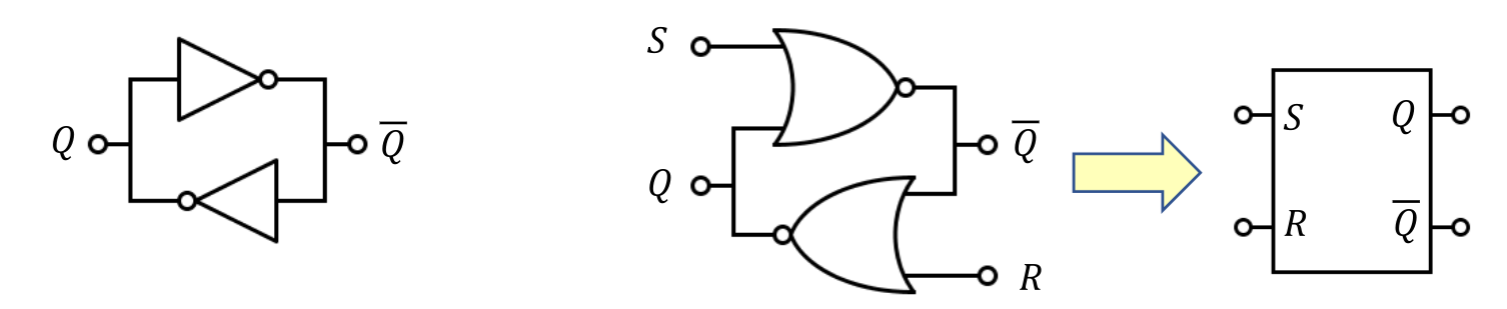
\includegraphics[scale=0.22]{../figures/sr_latch.png}
\end{center}

\end{document}
